\section{Question 2}

\begin{question}
    Analyze the impact of the minimal gain (using the gain ratio splitting criterion) and maximal depth
    parameters on the characteristics on the Decision Tree model learnt from the whole dataset (keep
    the default configuration for all the other parameters).
    \\
    Report at least 5 different screenshots showing Decision Trees (or portions of them) generated with
    different configuration settings.
\end{question}

\begin{answer}
    The impact of the \textbf{minimal gain} on the model affects the complexity(height) of it. As the figure 3 shows,
    with a value too high the model just predict a simple class for every input.
    With a value small, it reaches a height of max 6.
    When it reaches the height of 6, even if the value is decreses the model does not get more depth.
    \begin{figure}
        \centering
        \subfigure[]{
\includegraphics[width=0.48\textwidth]{Screenshot_4.png}}
        \subfigure[]{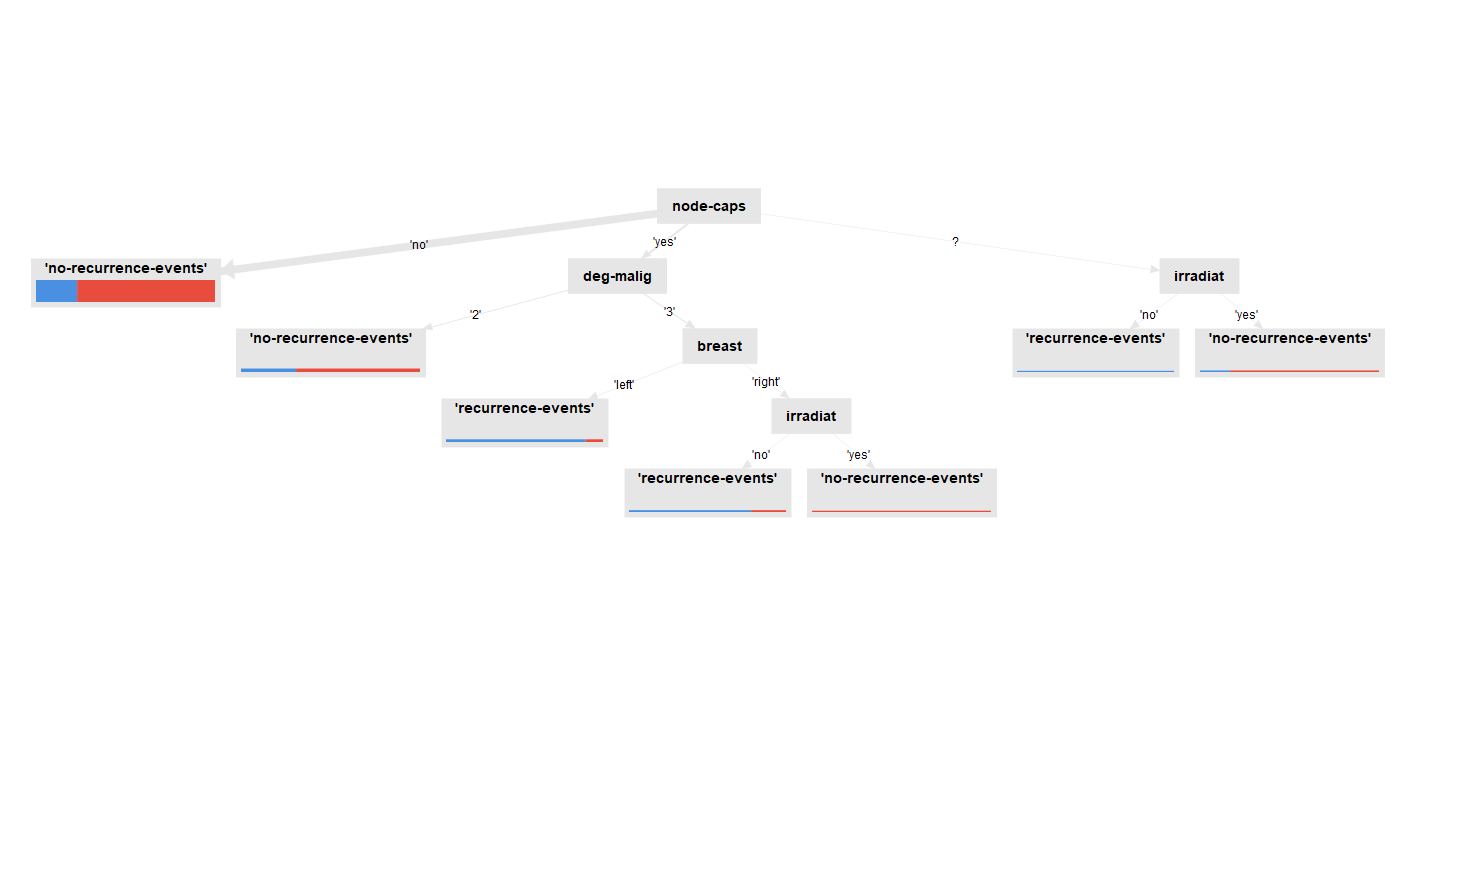
\includegraphics[width=0.48\textwidth]{Screenshot_5.png}}
        \subfigure[]{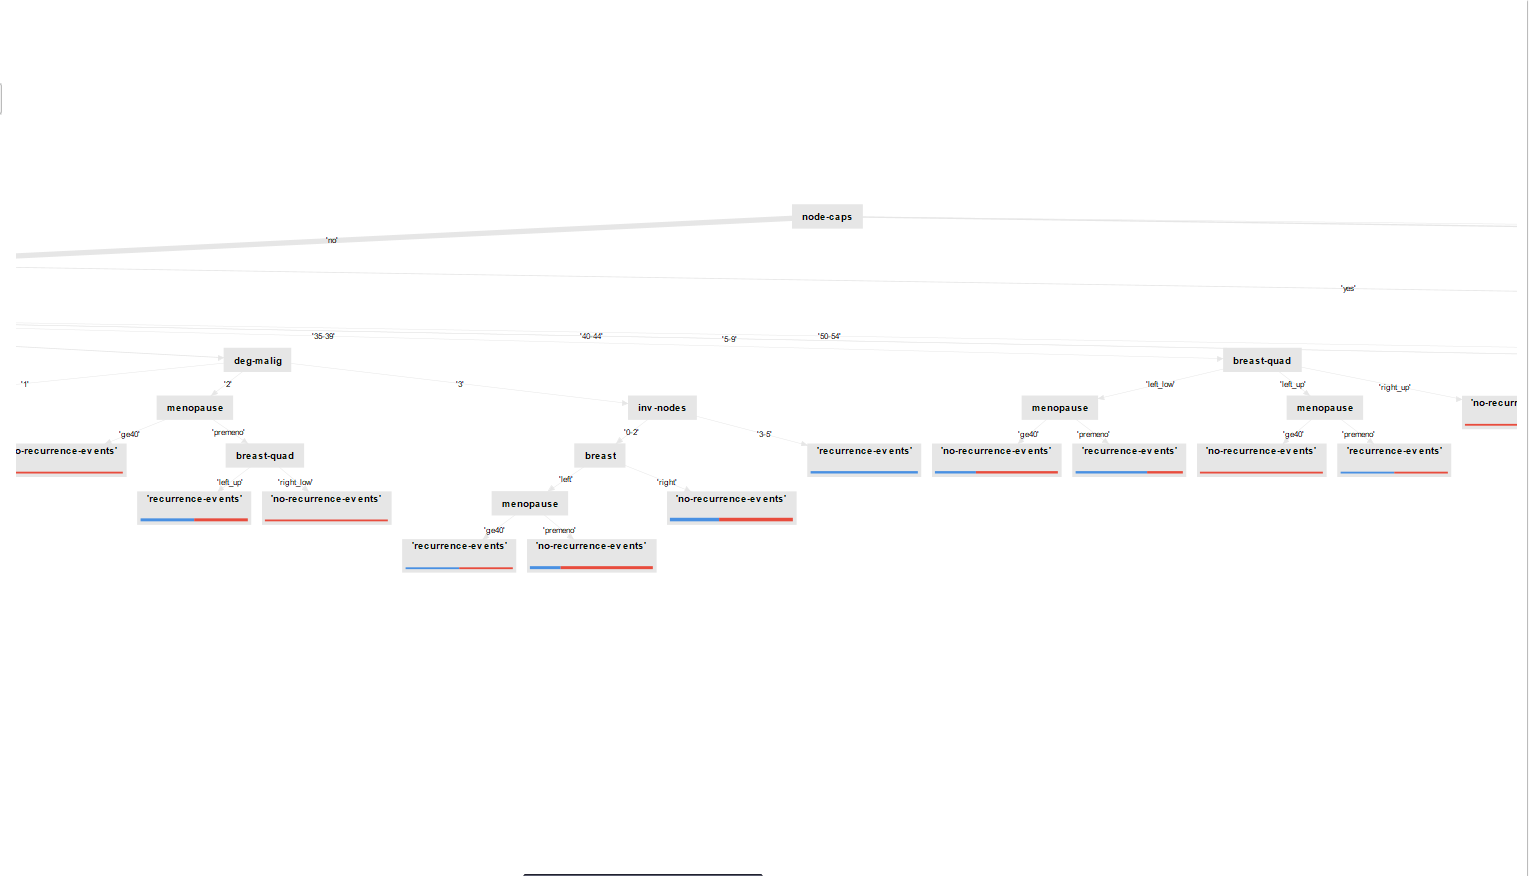
\includegraphics[width=0.48\textwidth]{Screenshot_6.png}}
        \subfigure[]{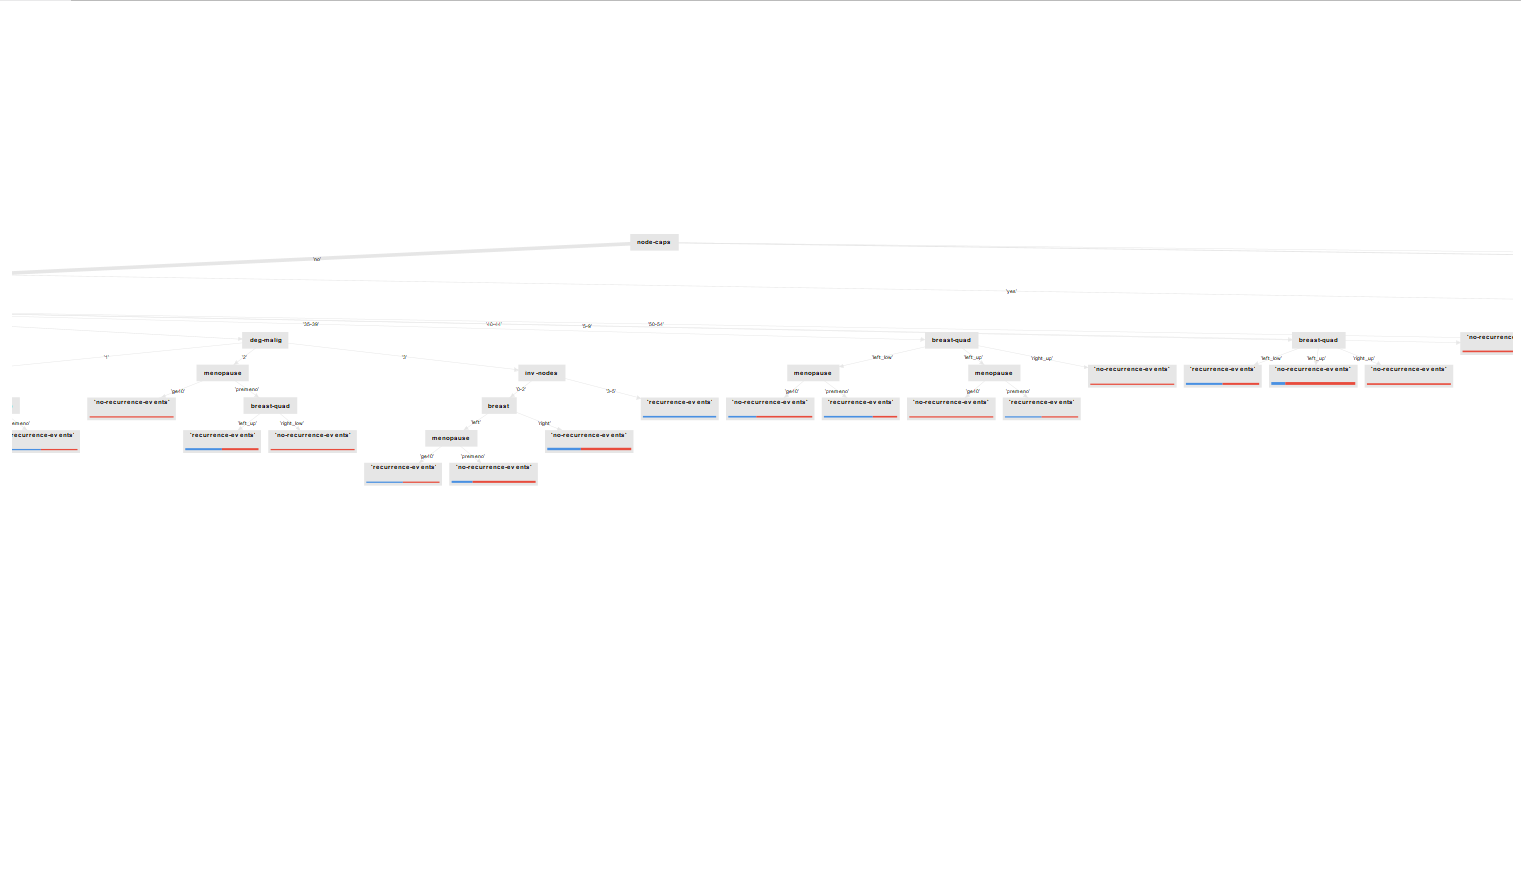
\includegraphics[width=0.48\textwidth]{Screenshot_7.png}}
        \caption{Impact of the \textbf{minimal gain} with values (maximal depth fixed to 1000)
        \\
            (a) 0.065 (b) 0.06 (c) 0.001 (d) 1x1e-5}
    \end{figure}
    \linebreak
    \\
    The impact of the \textbf{maximal depth} affects how depth the Decision Tree can go. For example with a
    \textbf{minimal gain} of 0.001, Figure 4 shows how the model stops when reaching the \textbf{maximal depth}.
    \begin{figure}
        \centering
        \subfigure[]{
\includegraphics[width=0.35\textwidth]{Screenshot_8.png}}
        \subfigure[]{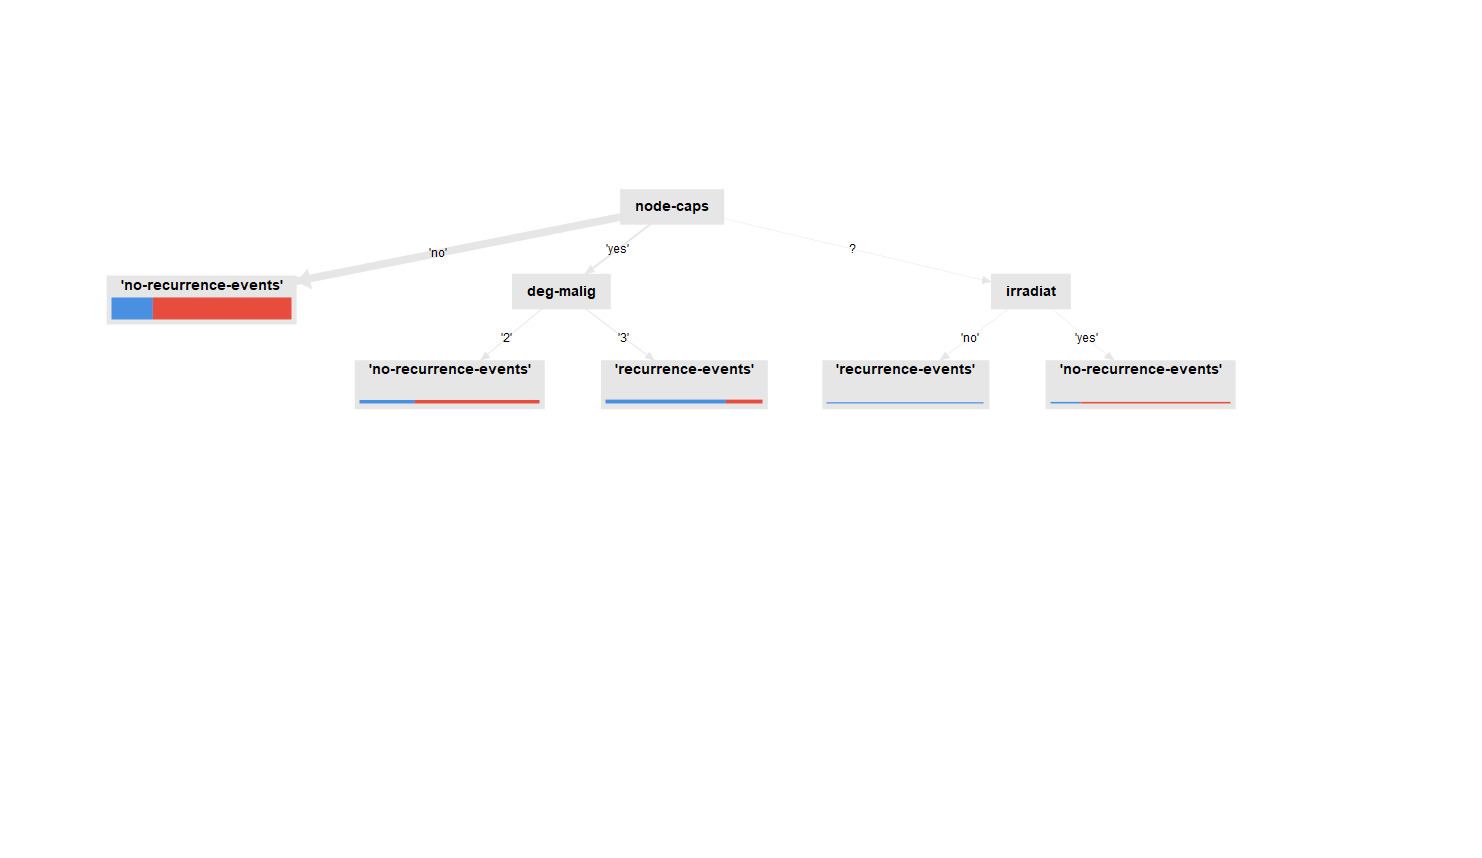
\includegraphics[width=0.35\textwidth]{Screenshot_9.png}}
        \subfigure[]{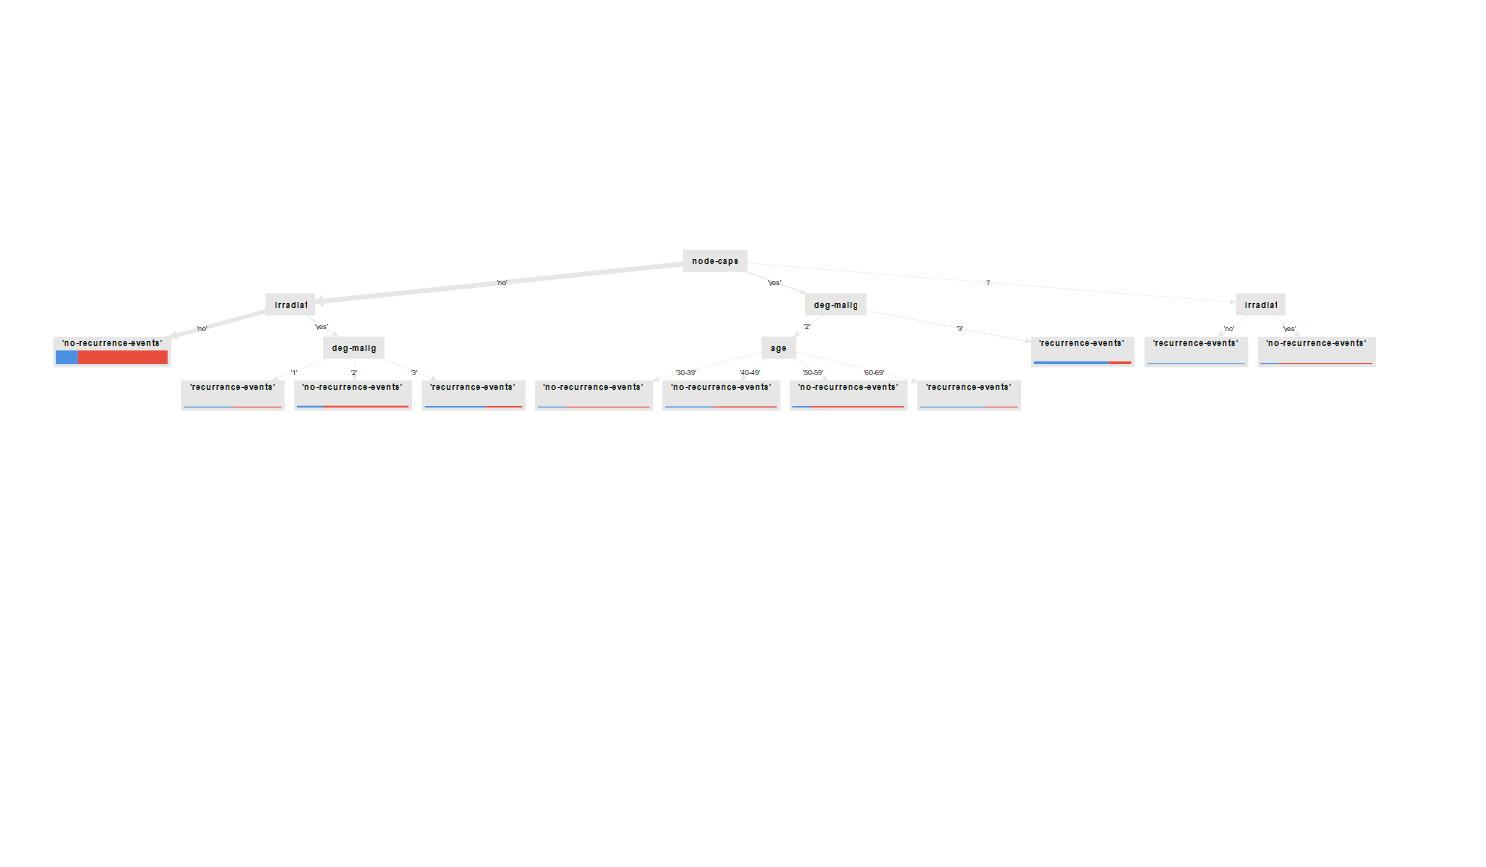
\includegraphics[width=0.35\textwidth]{Screenshot_10.png}}
        \subfigure[]{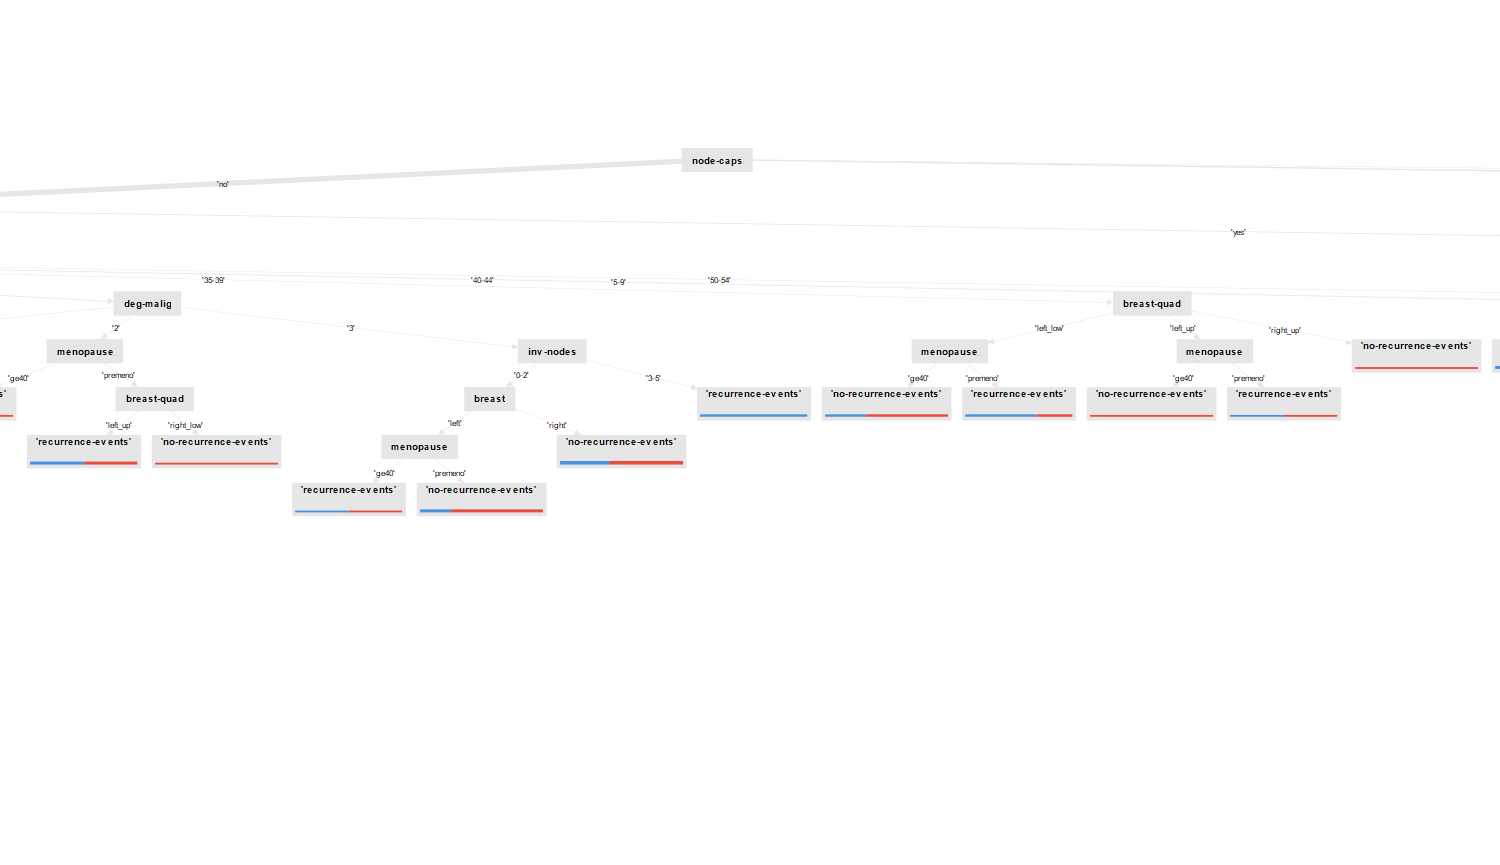
\includegraphics[width=0.35\textwidth]{Screenshot_11.png}}
        \caption{Impact of the \textbf{maximal depth} with values (minimal gain fixed to 0.001)
            \\
            (a) 1 (b) 3 (c) 4 (d) 1000}
    \end{figure}
    An important note is that \textbf{maximal depth} does not increases or reduces complexity. In the figure 5, there
    are two models with the same depth, one because it was restricted by \textbf{maximal depth} and other that was found
    setting \textbf{minimal gain} to 0.06. Even though both have a height of 5, the one with lower \textbf{minimal} is
    clearly more complex(more branches).
    \\
    \begin{figure}
        \centering
        \subfigure[]{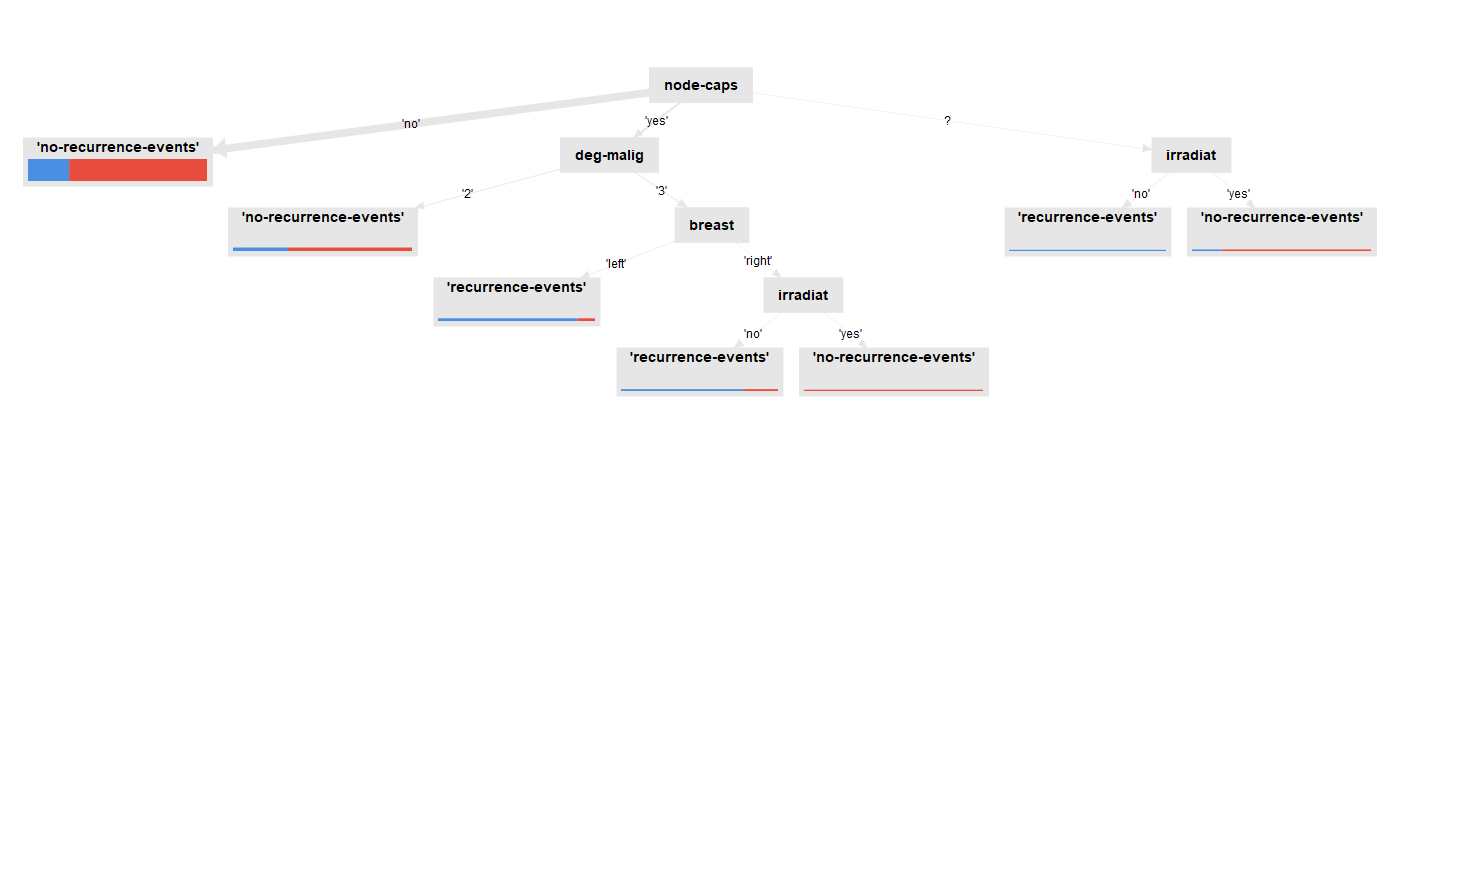
\includegraphics[width=0.35\textwidth]{Screenshot_13.png}}
        \subfigure[]{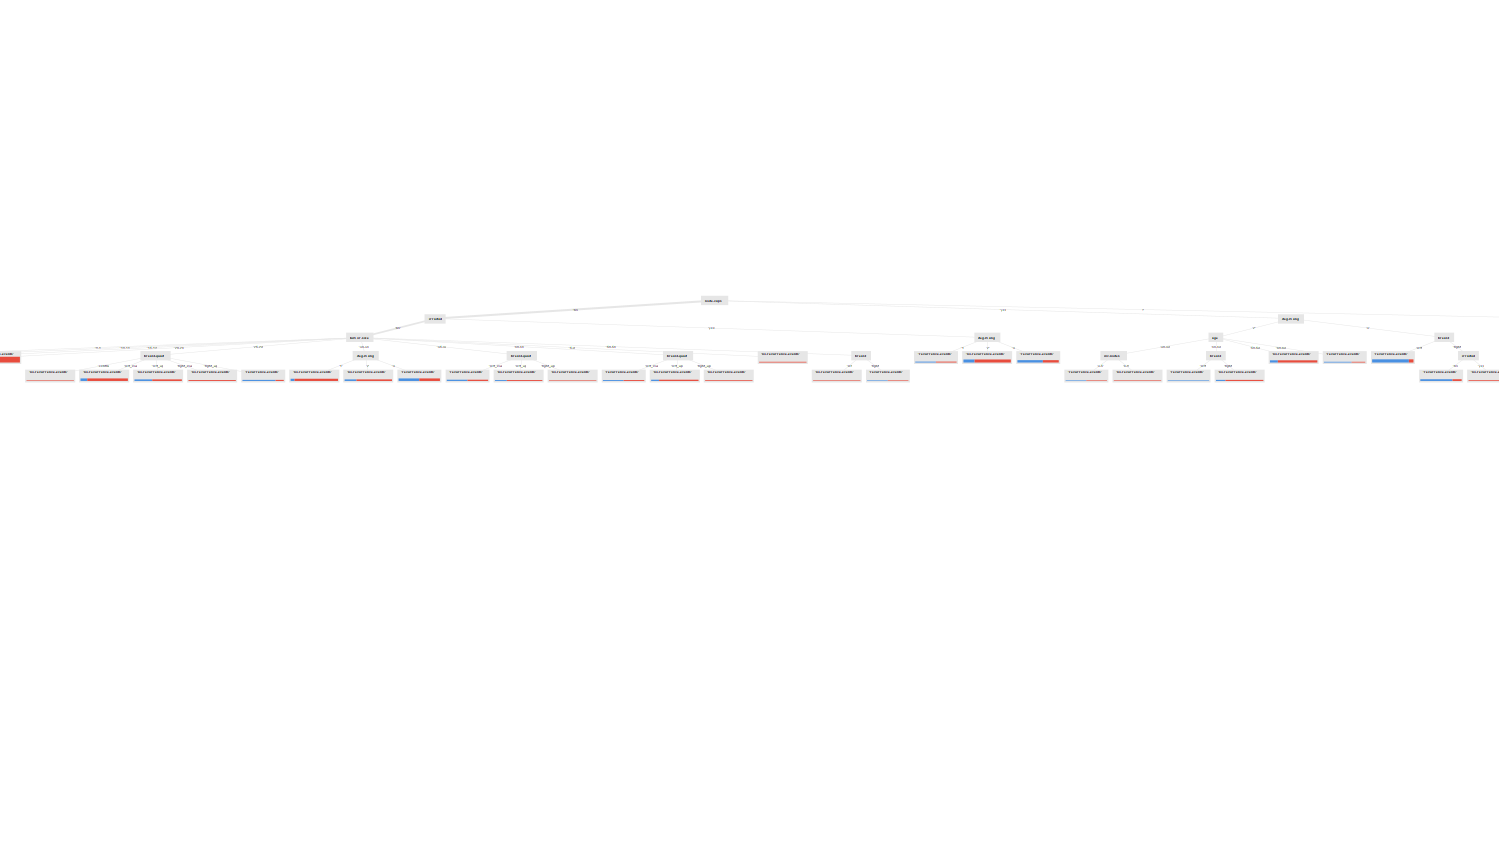
\includegraphics[width=0.35\textwidth]{Screenshot_14.png}}
        \caption{Impact of the \textbf{maximal depth} \textbf{minimal gain}
            \\
            (a) minimal gain: 0.06 maximal depth: 1000 (b) minimal gain: 1x10-5 maximal depth: 5}
    \end{figure}
\end{answer}
\pagebreak